\documentclass{article}
\usepackage{graphicx}
\usepackage{amsmath}
\usepackage{float}
\usepackage{amsfonts}
\usepackage{listings}
\usepackage{xcolor}
\usepackage[utf8]{inputenc}
\usepackage{hyperref}
\usepackage{fancybox}
\usepackage{booktabs}
\usepackage{array}
\usepackage{tikz}
\usepackage{amsfonts}
\usepackage{dsfont}
\usepackage{pgfplots}
\pgfplotsset{compat=1.18}
\usepackage[margin=2cm]{geometry}
\usepackage[french]{babel} % Pour les éléments en français
\usetikzlibrary{shapes, arrows.meta, positioning}
\usepackage[labelfont=bf, font=small]{caption}  % Pour personnaliser le titre de la figure


\title{HAX711X - Analyse des Données Multidimensionnelles \\ DM2 Classification automatique}
\author{SCAIA Matteo et MARIAC Damien}
\date{\today} 

\begin{document}

\maketitle

\begin{figure}[h] 
    \centering
    
\includegraphics[width=0.5\textwidth]{ssd_logo.png} 
\end{figure}

\begin{figure}[h] 
    \centering
    
\includegraphics[width=0.5\textwidth]{logo_um_2022_rouge_RVB.png} 
\end{figure}

\newpage

\tableofcontents

\newpage
\section{Treillis de Galois}
\subsection{Introduction}
Le treillis de Galois est une structure mathématique utilisée en analyse de données pour extraire des règles d’implication. Il est construit à partir de données décrites par des propriétés booléennes, permettant de représenter les relations entre ces propriétés et les ensembles d’objets associés. 
Le treillis de Galois peut également intégrer des relations liant les données entre elles.
\subsection{Interprétation et création du treillis de Galois}
Dans cette question, nous allons analyser le treillis de Galois construit à partir des données fournies par le sujet afin de modéliser les relations entre les films et leurs caractéristiques.
\begin{figure}[h]
    \centering
    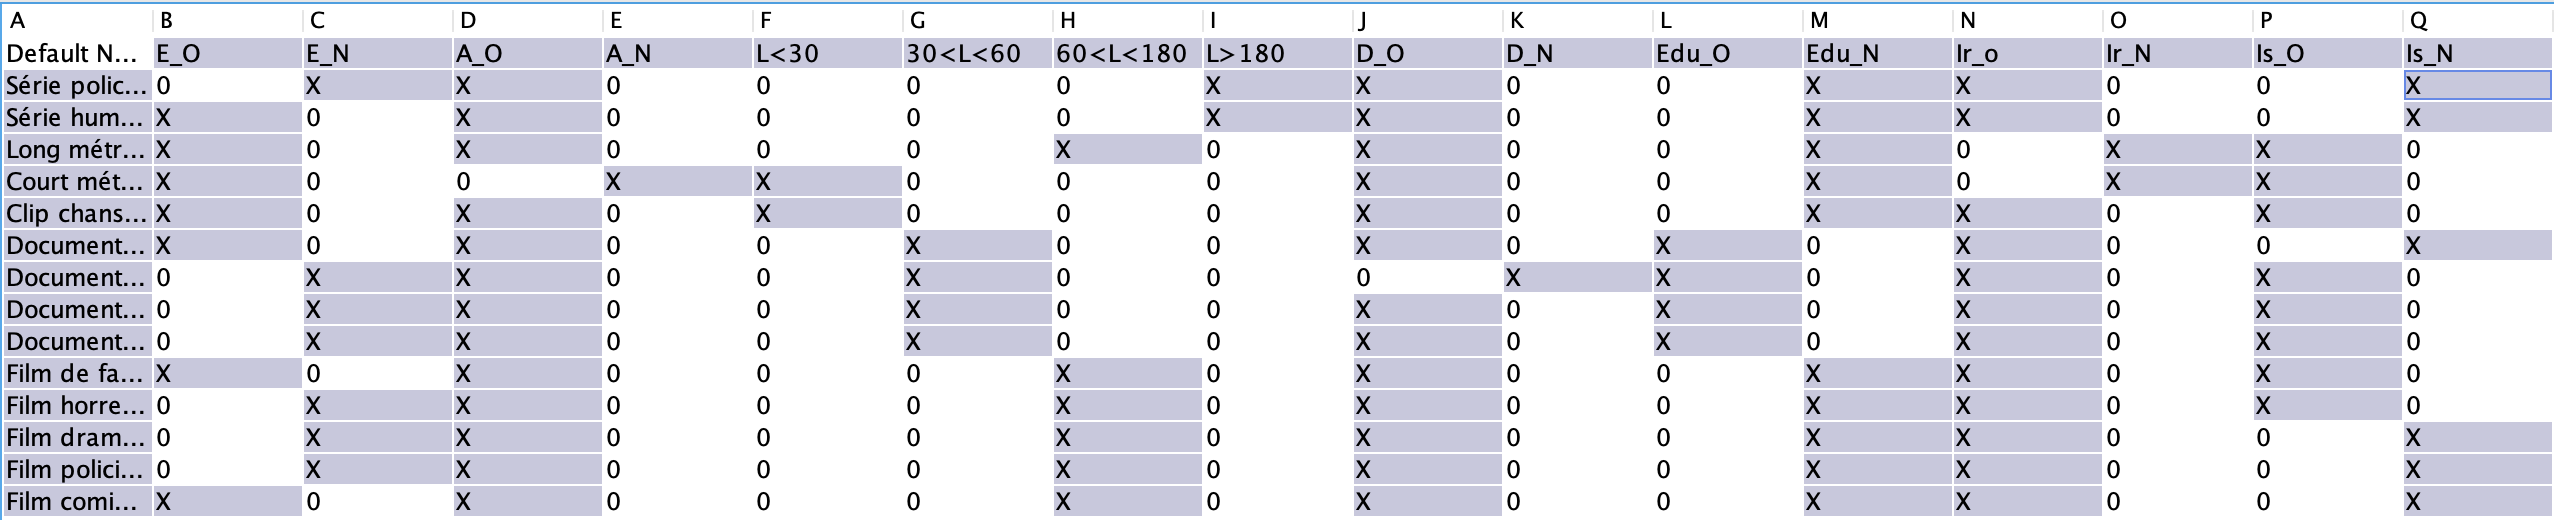
\includegraphics[width=0.7\textwidth]{tableau.png}
    \caption{Tableau des relations binaires}
    \label{fig:tableau} 
\end{figure}
\\
À l'aide du logiciel Galicia, nous obtenons le treillis de Galois suivant :
\begin{figure}[h]
    \centering
    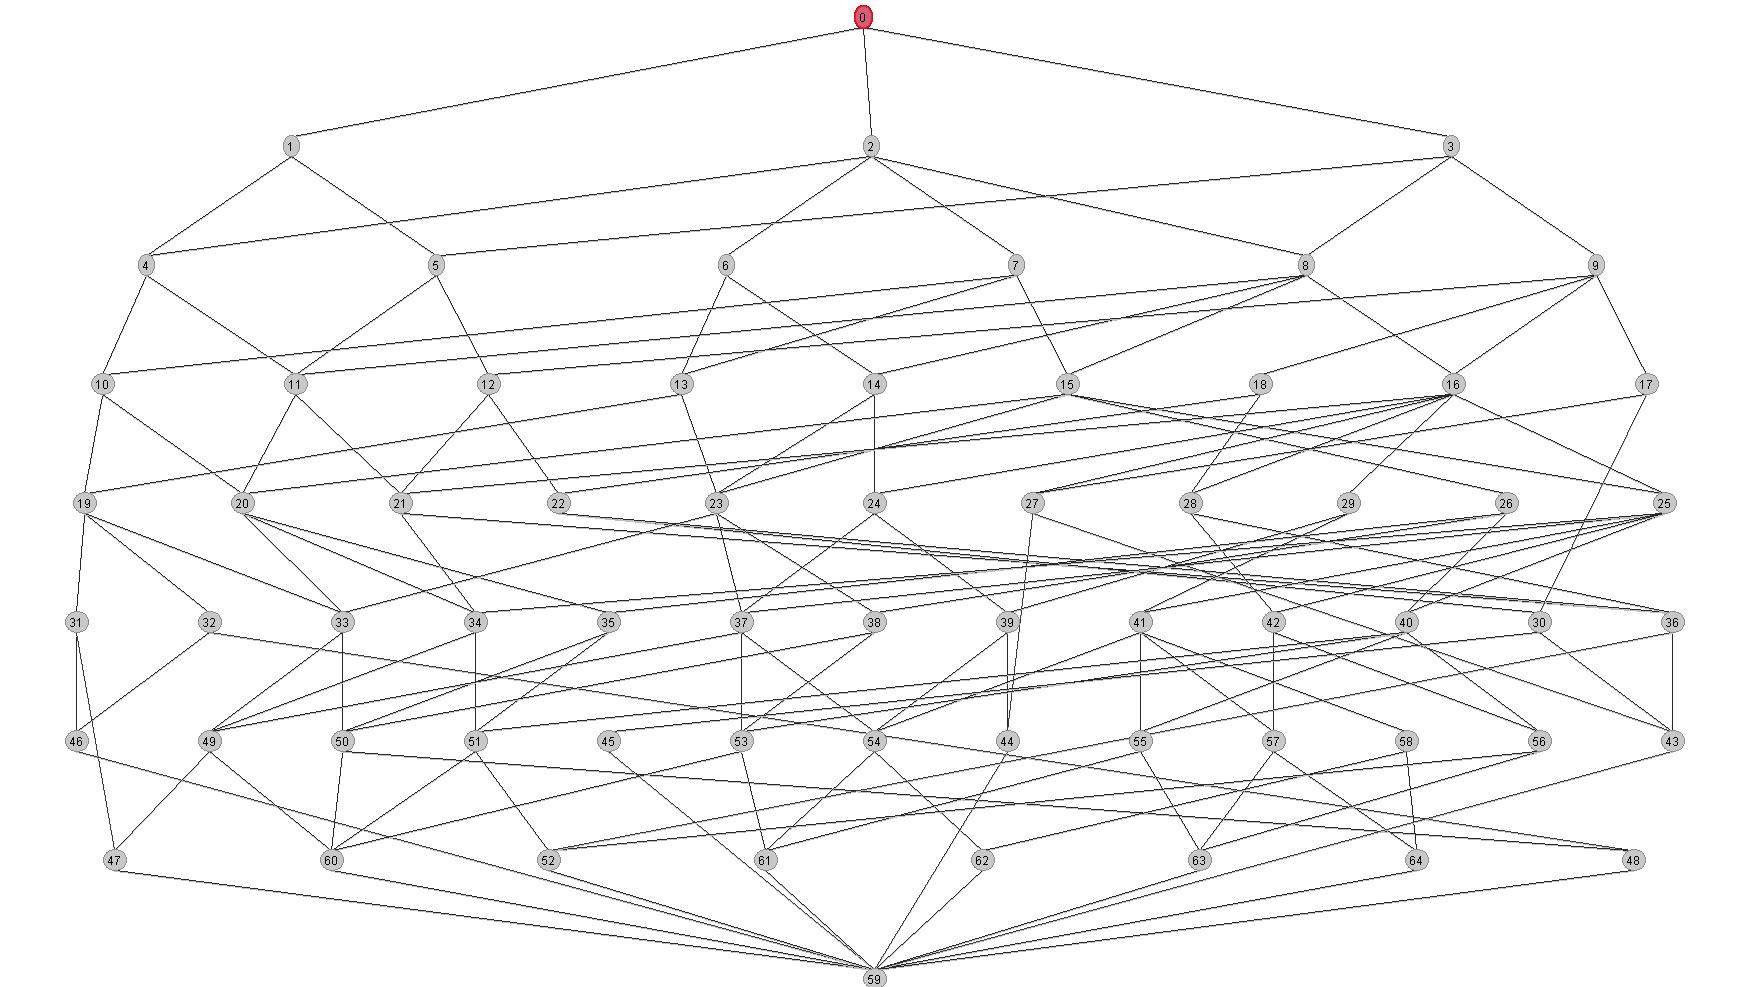
\includegraphics[width=0.7\textwidth]{treillis.png}
    \caption{Treillis de Galois de notre tableau}
    \label{fig:treillis} 
\end{figure}
\\
Dans un treillis de Galois, les nœuds situés aux extrémités correspondent soit à l’ensemble de tous les individus (en haut), soit à l’ensemble de toutes les caractéristiques (en bas). Ces nœuds étant trop généraux ou trop spécifiques, leur analyse n’est pas nécessaire.
\\
\\
Le nœud 57 regroupe les films dramatiques (FD), les films policiers (FP) et les séries policières (SP), caractérisés par les propriétés suivantes : ils s’adressent aux adolescents et aux adultes (A = Oui), ont un objectif distractif (D = Oui), ne sont pas éducatifs (ED = Non), ne ciblent pas les enfants (E = Non), utilisent des images réelles (IR = Oui) et n’incluent pas d’images de synthèse (IS = Non). Ce regroupement correspond à des œuvres qui partagent des thématiques et des intentions narratives du genre "thriller".
\\
Par ailleurs, ce nœud est lié à la classe 42, qui partage les mêmes caractéristiques mais inclut également des œuvres utilisant des images de synthèse. Cela permet d’y intégrer des films d’horreur (FH).
\\
Cette classe peut être interprétée comme un regroupement de film conçues pour provoquer du suspense ou des "frissons".
\\
\\
Le nœud 16 représente une classe large regroupant plusieurs types de films et séries partageant diverses caractéristiques : un public adulte, une vocation distractive, et des images réelles. Ce nœud est particulièrement intéressant, car il se connecte à plusieurs autres classes. Ces caractéristiques sont partagées par des genres variés. De ce fait, cette classe regroupe de nombreux types de films et séries, tels que les clips musicaux, les documentaires artistiques, les documentaires sur la nature, les documentaires scientifiques, les films comiques, les films dramatiques, les films de fantasy, les films d’horreur, ainsi que les séries humoristiques et policières.
\\
\\
On remarque également le nœud 17, qui regroupe tous les documentaires. Les caractéristiques de cette classe sont qu’elle s’adresse aux adultes (A = Oui), a une vocation éducative (ED = Oui), utilise des images réelles (IR = Oui) et correspond à des productions de courte durée (30-60 minutes). Ces caractéristiques décrivent ce que sont les documentaires.
\\



\section{Classification hiérarchique de parcelles forestières tropicales}
Charger dans le logiciel les données relatives au peuplement arboré de la forêt du bassin du Congo
(Datagenus.csv). Inspectez le fichier et corrigez-en les erreurs triviales s'il en est. Ces données fournissent
sur 1000 parcelles de cette forêt: les variables de comptage de 27 espèces d'arbres (gen1, ..., gen27), la
surface de la parcelle, le type forestier (forest) tel qu'identifié par les écologues . On ne tiendra pas compte
des autres variables. Calculer la densité de peuplement de chaque espèce par unité de surface pour les 1000
parcelles. Les parcelles seront traduits en nuage dans l'espace des 27 densités de peuplement.

L4.2 -> justification a l'oral : 1 min
\subsection{Préparation des données}
\label{Q1}
Nous traduisons les observations dans l’espace euclidien, où la distance servira de mesure de dissimilarité globale entre les parcelles. Cette mesure repose sur la comparaison des écarts sur les différentes dimensions (densités des espèces). Puisque toutes les dimensions (espèces) sont supposées avoir une importance équivalente, aucune ne doit dominer le calcul.
\\
On note $x_i$ la $i$-ième parcelle. La distance euclidienne entre deux parcelles $x_1$ et $x_2$ est :  
\[
d(x_1, x_2) = \sqrt{\sum_{j=1}^{27} (x_1^j - x_2^j)^2}
\]
où \( x_1^j \) et \( x_2^j \) représentent respectivement la densité de l'espèce j dans les parcelles 1 et 2.
\\
En analysant la contribution de chaque espèce, nous obtenons le tableau suivant :
\begin{table}[h!]
    \centering
    \caption{Contribution des espèces (gen1 à gen11)}
    \label{tab:pourcentage}
    \begin{tabular}{@{}l*{11}{c}@{}}
    \toprule
     & gen1 & gen2 & gen3 & gen4 & gen5 & gen6 & gen7 & gen8 & gen9 & gen10 & gen11 \\ 
    \midrule
    Pourcentage & 
    0.23 & 0.00 & 0.03 & 0.00 & 0.01 & 0.05 & 0.00 & 64.90 & 0.07 & 0.48 & 1.03 \\ 
    \bottomrule
    \end{tabular}
    \end{table}
\\
Nous voyons que les variables ne contribuent pas tous de la même manière. Les contributions des espèces gen1 à gen27 à la distance euclidienne ne sont pas uniformes. Par exemple, gen8 représente 64.90 \% de la distance, ce qui montre que les variations dans cette dimension dominent les calculs de dissimilarité.
\\
Nous standardisons les densités de peuplement et on note \( \mathbf{Z} \) la matrice associée :

\[
z_i^j = \frac{x_i^j - \overline{x}^j}{\sigma_{x^j}}
\]
avec \( x_i^j \) la densité de l’espèce \( j \) sur la parcelle \( i \), \( \overline{x}^j \) la moyenne des densités pour l’espèce \( j \), et \( \sigma_{x^j} \) l’écart-type de l’espèce \( j \).\\
La standardisation assure que chaque dimension contribue de manière équivalente à la mesure de la dissimilarité, indépendamment de son échelle initiale ou de sa variabilité.
\subsection{CAH des parcelles sur les densités de peuplement}
À partir des données contenant les densités de peuplement obtenues à la question \ref{Q1} et standardisées, nous allons procéder à une classification des parcelles en fonction de leur peuplement arboré. 
L’objectif est de regrouper les parcelles en classes homogènes et de déterminer le nombre optimal de classes.
\\
Intéressons-nous à la classification automatique avec l'indice de Ward.
\\\\
\textbullet\ \underline{Indice de Ward}\\
En utilisant le code en langage R fournies dans le sujet, nous pouvons réaliser une classification ascendante hiérarchique. L’objectif est de déterminer le nombre optimal de classes prometteuses.
Nous obtenons le dendogramme suivant :
\begin{figure}[h]
    \centering
    \includegraphics[width=0.8\textwidth]{wardC2.png}
    \caption{Dendogramme (indice de Ward)}
    \label{fig:Ward} 
\end{figure}
\\
Nous avons choisi de couper en 8 classes.
\end{document}